\documentclass{article}
\usepackage[a4paper, margin=25mm]{geometry}
\usepackage{tikz}
\usepackage[utf8]{inputenc}
\usepackage{mathptmx}
\usepackage{hyperref}
\usepackage{xcolor}
\usepackage{wrapfig}

\newcommand{\insertTitle}{Website Design}

\begin{document}
\begin{center} \fontsize{35}{0} \textit{Università degli studi di Salerno} \\
\fontsize{20}{0} \textit{\textbf{Corso di Laurea in Informatica}}
\end{center}
\begin{tikzpicture}[remember picture, overlay]
  \node[opacity=0.6,inner sep=0pt] at (current page.center)
   {
\includegraphics[scale=1.5]{logo_standard.png}};
\end{tikzpicture}

\newpage
\begin{center} 
    \fontsize{28}{0} \textit{\textbf{PROGRAMMAZIONE WEB}}
    \\[2cm]
    \fontsize{28}{0} \textit{\textbf{\insertTitle}}
    \\[2cm]
    \fontsize{36}{0} \textit{\textbf{“TeraWare”}}
    \\[5cm]
    \begin{table}[h]
        \centering
        \begin{tabular}{lllll}
        \multicolumn{1}{c}{\huge\textbf{Docente:}} &  &  & \multicolumn{2}{c}{\huge Studenti:} \\
        \multicolumn{1}{c}{\large Rita Francese}     &  &  & \textit{\large \textbf{Nome}} & \textit{\large\textbf{Matricola}} \\
                          &  &  & \large Antonio Scognamiglio   & \large . \\
                          &  &  & \large Giovanni Scorziello & \large . \\
                          & & & \large Manuela Esposito & \large . \\
                          & & & \large Domenico Antonio Gioia & . \large 
        \end{tabular}
    \end{table}
\end{center}
\newpage
\begin{center}
    \fontsize{28}{0} \textit{Anno Accademico: 2020/21}
\end{center}
\begin{large}
\tableofcontents
\newpage 
\begin{center}
    \fontsize{36}{0} \textit{\textbf{TeraWare}}
\end{center}
\section{Obiettivo del progetto}
\textbf{TeraWare} è un sito di ecommerce specializzato nella vendita di prodotti hardware e software legati all'informatica, in particolare per il \textit{gaming} e per \textit{l'ufficio}. L'obiettivo è fornire attrezzature con performance elevate per garantire la massima resa in ambito professionale. Il \textit{gaming} è un trend in crescita negli ultimi anni soprattutto grazie alla diffusione degli sport elettronici (\textit{esports}), che stanno diventando sempre più popolari per via dei riconoscimenti dagli enti nazionali\footnote{https://fide.gg/}.


Come per il gaming, anche per l'ufficio TeraWare offre molte soluzioni ad alte prestazioni per essere utilizzate nell'ambito della grafica, del disegno tecnico, montaggio video e molto altro.


Per permettere una navigazione ottimale sia da smartphone, tablet e desktop, il sito è realizzato in modo responsive per adattarsi alla dimensione dello schermo su cui è visualizzato. 
\section{Analisi di siti esistenti}
\subsection{AKInformatica}

\begin{center}
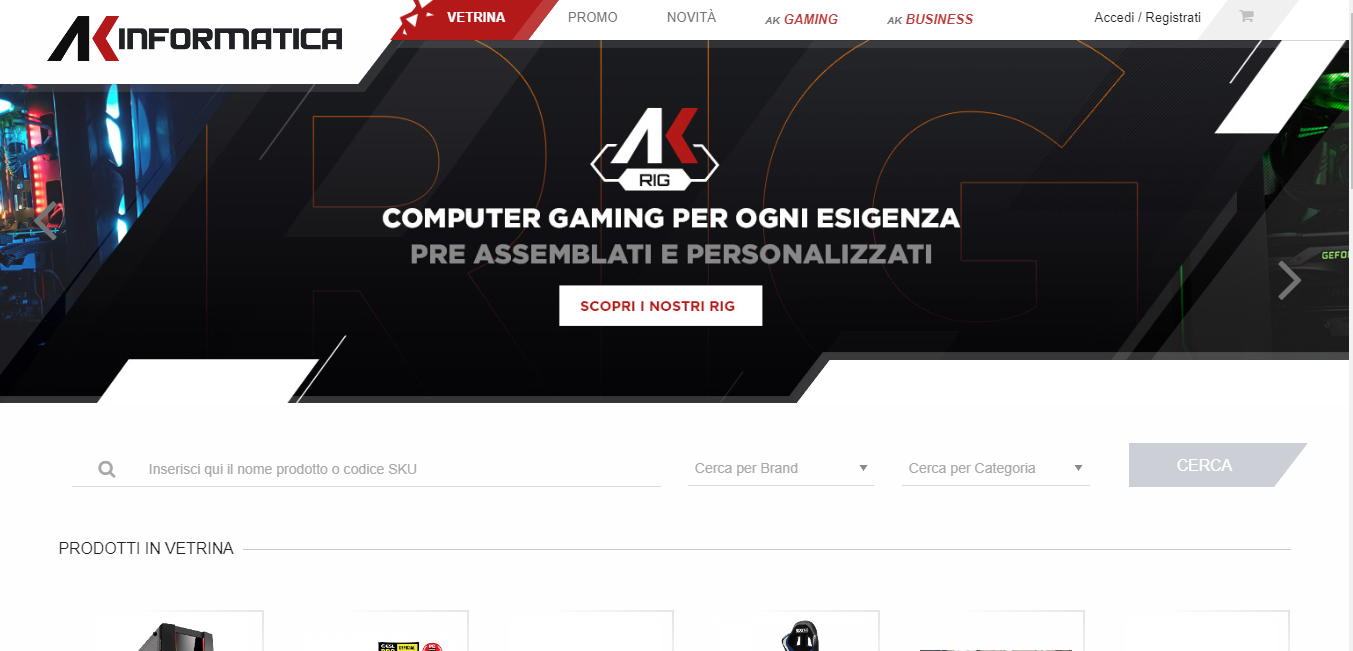
\includegraphics[scale=0.45]{akinformatica/ak1.png}
\end{center}
\href{https://shop.akinformatica.it/}{\underline{AKInformatica}} è un sito italiano di ecommerce, tra i più popolari nell'ambito del gaming. La homepage è composta da una presentazione di banner, che mostra offerte e novità. In alto per rendere facile la navigazione è presente una barra con dei pulsanti per navigare alle varie sezioni del sito (\textit{Vetrina, Promo, Novità, Gaming, Business}). Inoltre ci sono diverse caselle di testo per cercare i prodotti per nome, brand o categoria. Al di sotto c'è la vetrina prodotti, in cui vengono mostrati gli articoli più acquistati.


Non si possono aggiungere al carrello prodotti senza registrarsi, e non è possibile registrarsi con un provider di autenticazione (\textit{Facebook, Google...}) \\ \\


Nel footer del sito troviamo i metodi di pagamento e le informazioni di contatto.
\begin{center}

\includegraphics[scale=0.45]{akinformatica/ak2.png}
\end{center}
\subsection{PC Hunter}
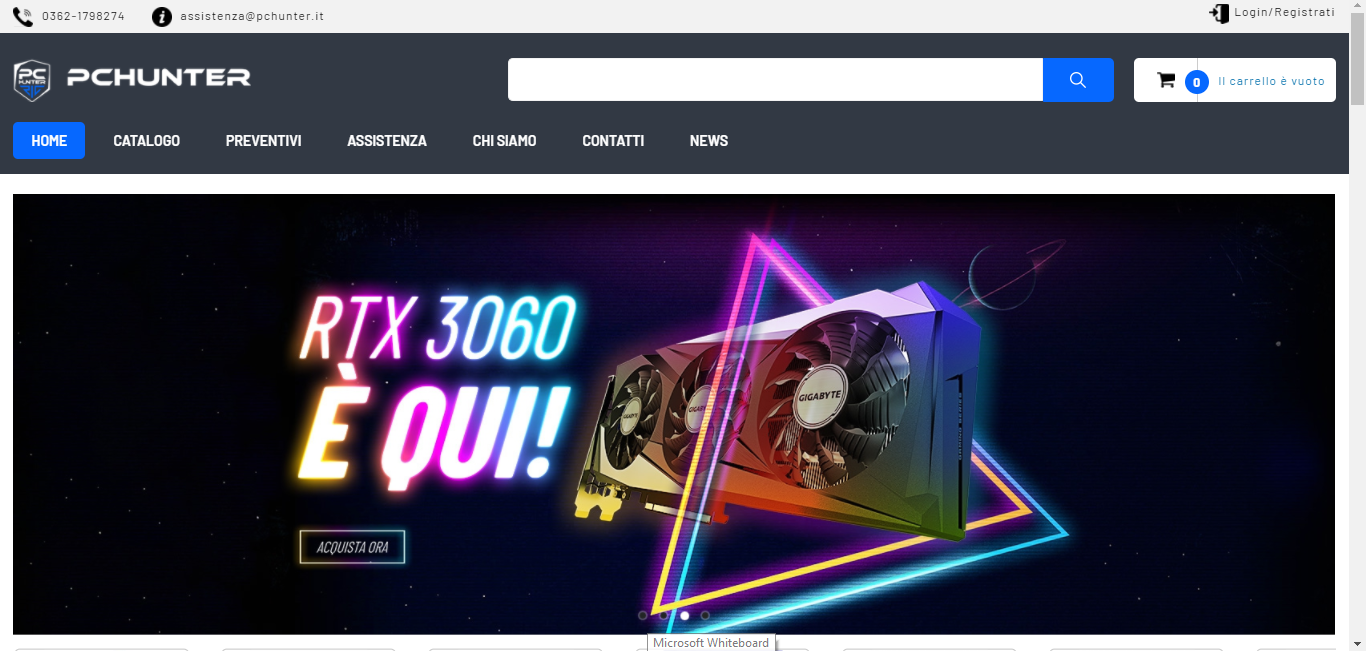
\includegraphics[scale=0.45]{pchunter/pchunter1.png}
Anche \href{https://www.pchunter.it/}{\underline{PC Hunter}} è uno dei top brand italiani per quanto riguarda l'ecommerce di periferiche informatiche di elevato livello. Nella homepage, diversamente da prima, in alto troviamo le informazioni di contatto, seguono la barra di ricerca, il pulsante per accedere al carrello e la barra di navigazione; l'utente può aggiungere prodotti allo \textit{shopping cart} senza registrazione, e accanto alla barra di ricerca verrà mostrato il totale dei prodotti che si ha intenzione di acquistare. Per procedere all'acquisto in ogni caso bisogna registrarsi.\\
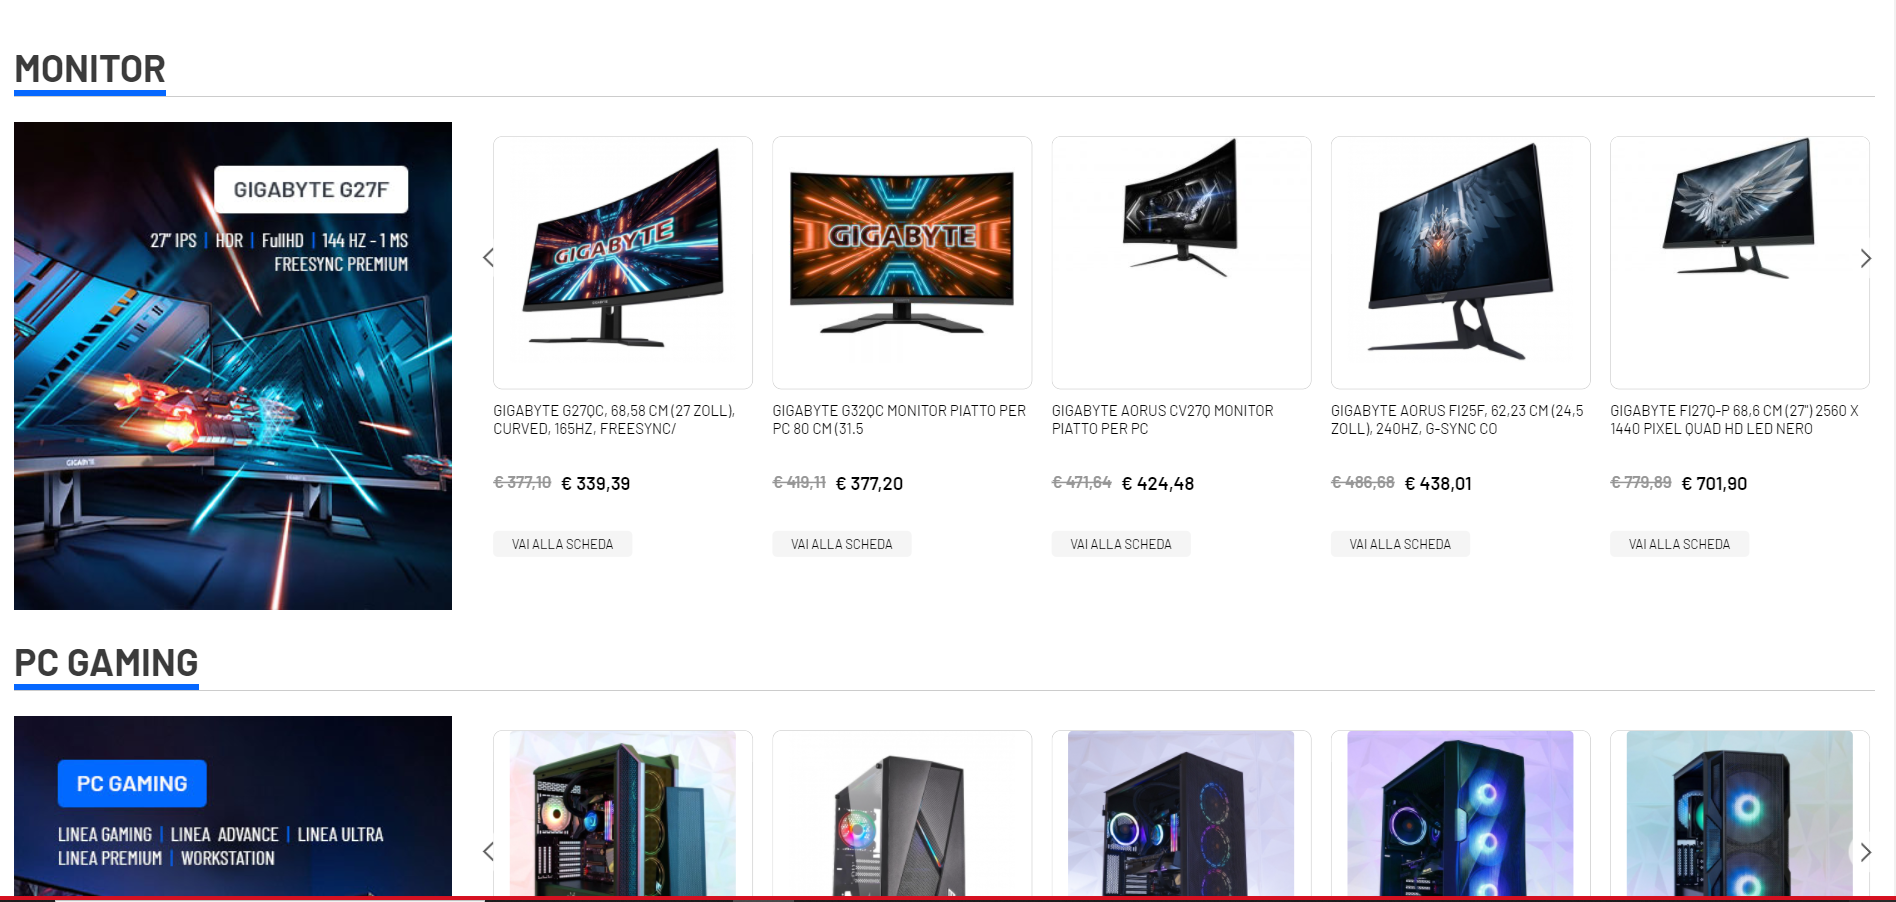
\includegraphics[scale=0.40]{pchunter/pchunter2.png}
Qui gli articoli sono disposti per categoria, offrendo una visualizzazione ordinata, con un'immagine rappresentativa a sinistra e la lista di prodotti che scorre orizzontalmente.
\section{Funzionalità del sito}
\subsection{Funzionalità amministrative}
\begin{itemize}
    \item Gestione degli articoli in vendita (aggiungi, rimuovi...)
    \item Gestione ordini
    \begin{itemize}
        \item Visualizzazione per data, ricerca degli ordini per cliente
    \end{itemize}
    \item Gestione codici coupon
\end{itemize}
\subsection{Funzionalità utente registrato}
    \begin{itemize}
        \item Aggiungere e rimuovere elementi dal carrello
        \item Completare un acquisto
        \item Visualizzare la lista degli ordini effettuati ordinata per data
        \item Modificare i propri dati anagrafici e le informazioni di pagamento
        \item Ricercare componenti per nome o per categoria
        \item Possibilità di aggiungere una recensione ai prodotti acquistati
        \item Visualizzazione feed di articoli consigliati dopo l'acquisto di un prodotto
        \end{itemize}
\subsection{Funzionalità utente guest}
    \begin{itemize}
        \item Aggiungere e rimuovere gli elementi dal carrello
        \item Ricercare componenti per nome o per categoria
        \item Per completare un acquisto è necessario registrarsi (è prevista la possibilità di registrazione anche in precedenza al \textit{checkout})
    \end{itemize}
    \section{Utenti del sito}
    Gli utenti del sito sono \textit{Amministratore, Utente registrato, Utente guest}
    \section{Diagramma navigazionale}
        \begin{center}
            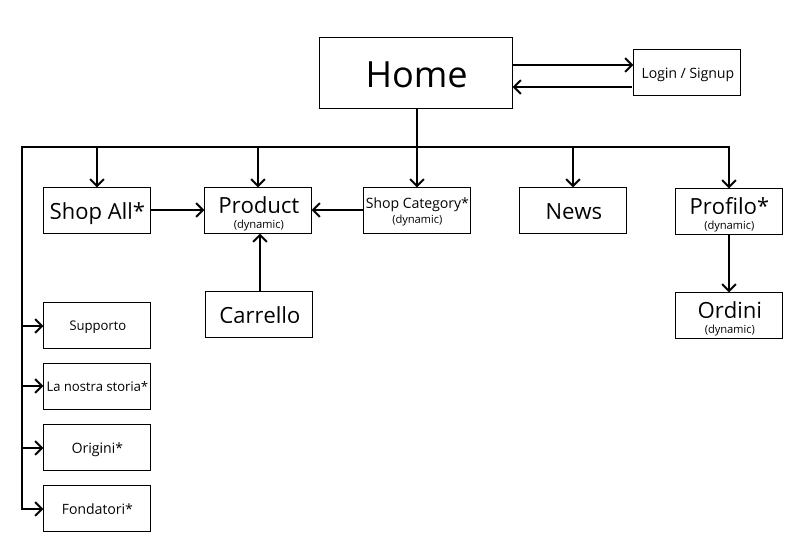
\includegraphics[scale=0.5]{teraware/_diagnavigazionale.png}
        \end{center} 
        Le pagine con \textit{*} sono raggiungibili tramite la navbar, quindi da qualunque pagina del sito.
    \section{Mappa dei contenuti}
        \begin{center}
            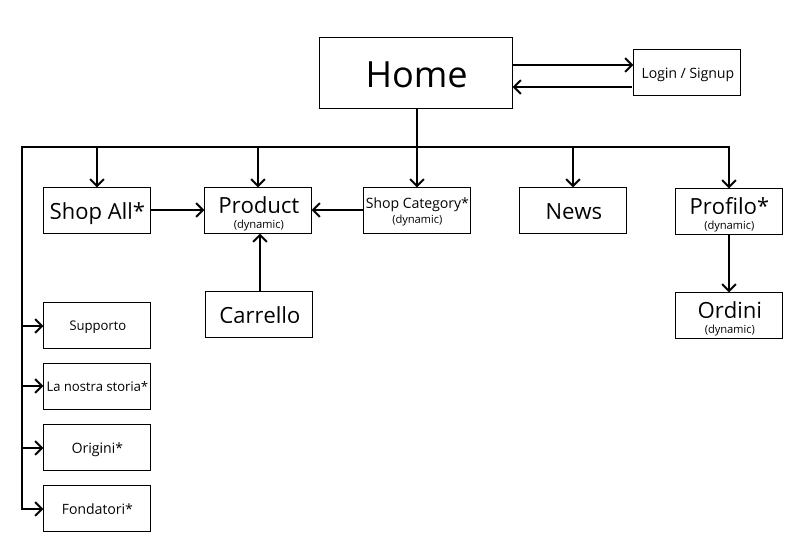
\includegraphics[scale=0.5]{teraware/_diagnavigazionale.png}
        \end{center}
        La pagina \textit{"supporto"} contiene alcune informazioni per i clienti in merito a resi, domande frequenti e \textit{Privacy Policy}. \textit{"La nostra storia, origini, fondatori e supporto"} sono pagine statiche che contengono paragrafi in merito alla storia e agli autori del progetto.
    \section{Base di dati}
        \begin{center}
        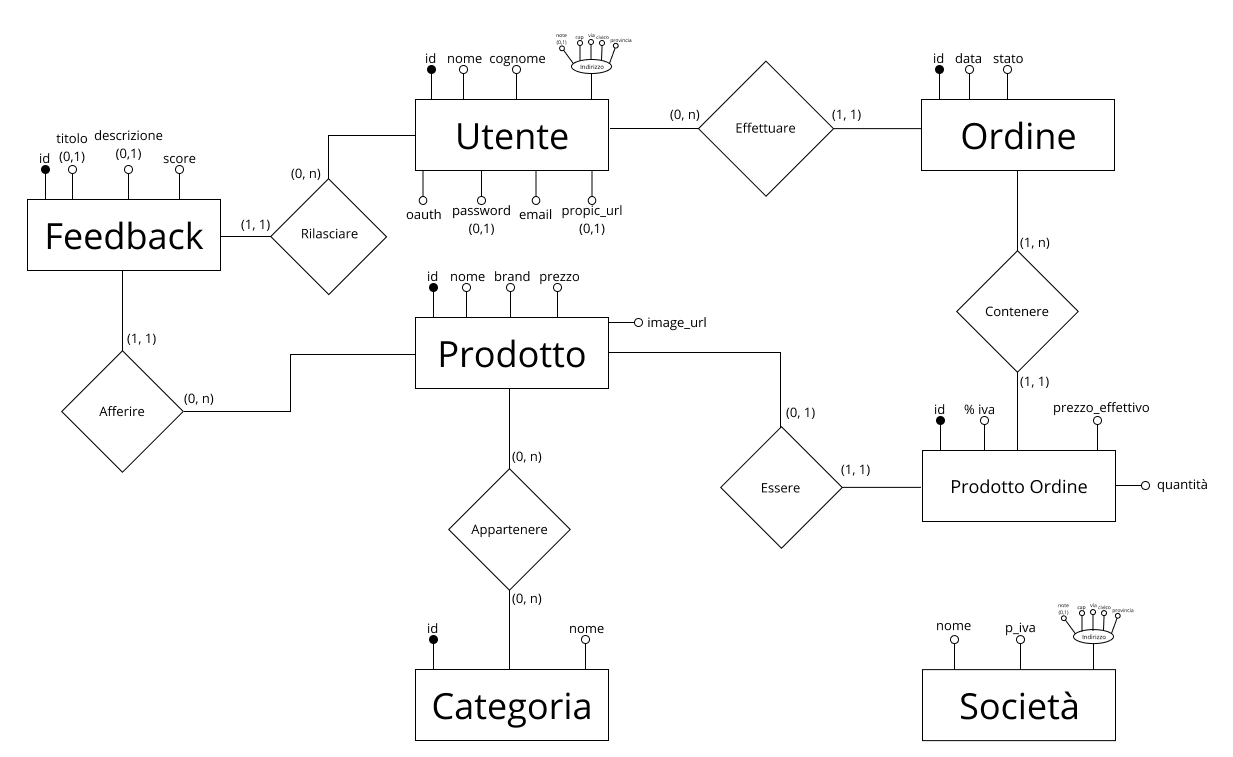
\includegraphics[scale=0.4]{teraware/er.png}
        \end{center}
    \section{Layout}
        \subsection{Home}
            \begin{center}
                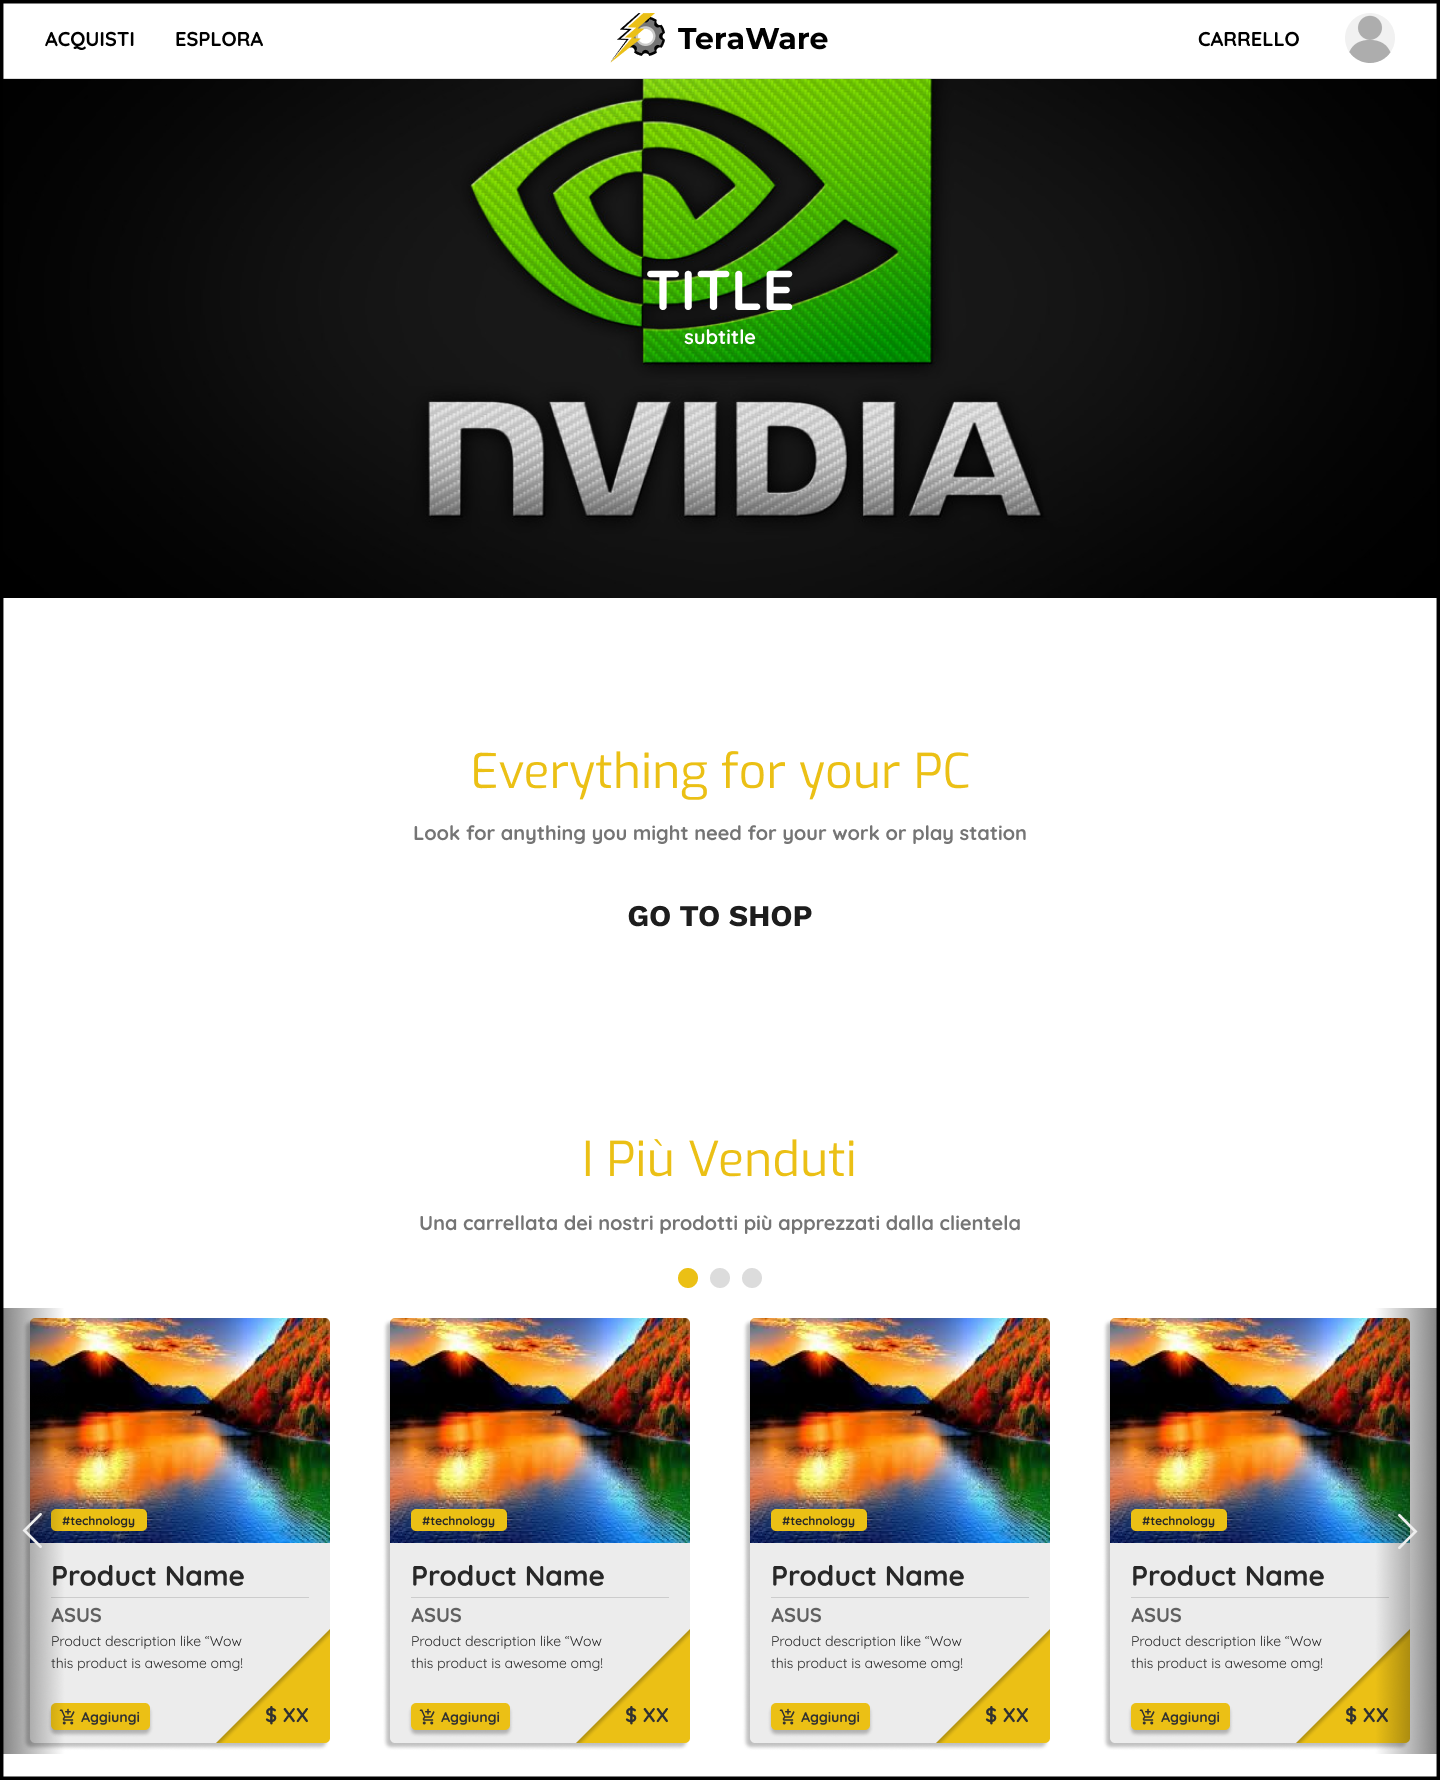
\includegraphics[scale=0.29]{teraware/_layouthome.png}
            \end{center}
        \subsection{News}
            \begin{center}
                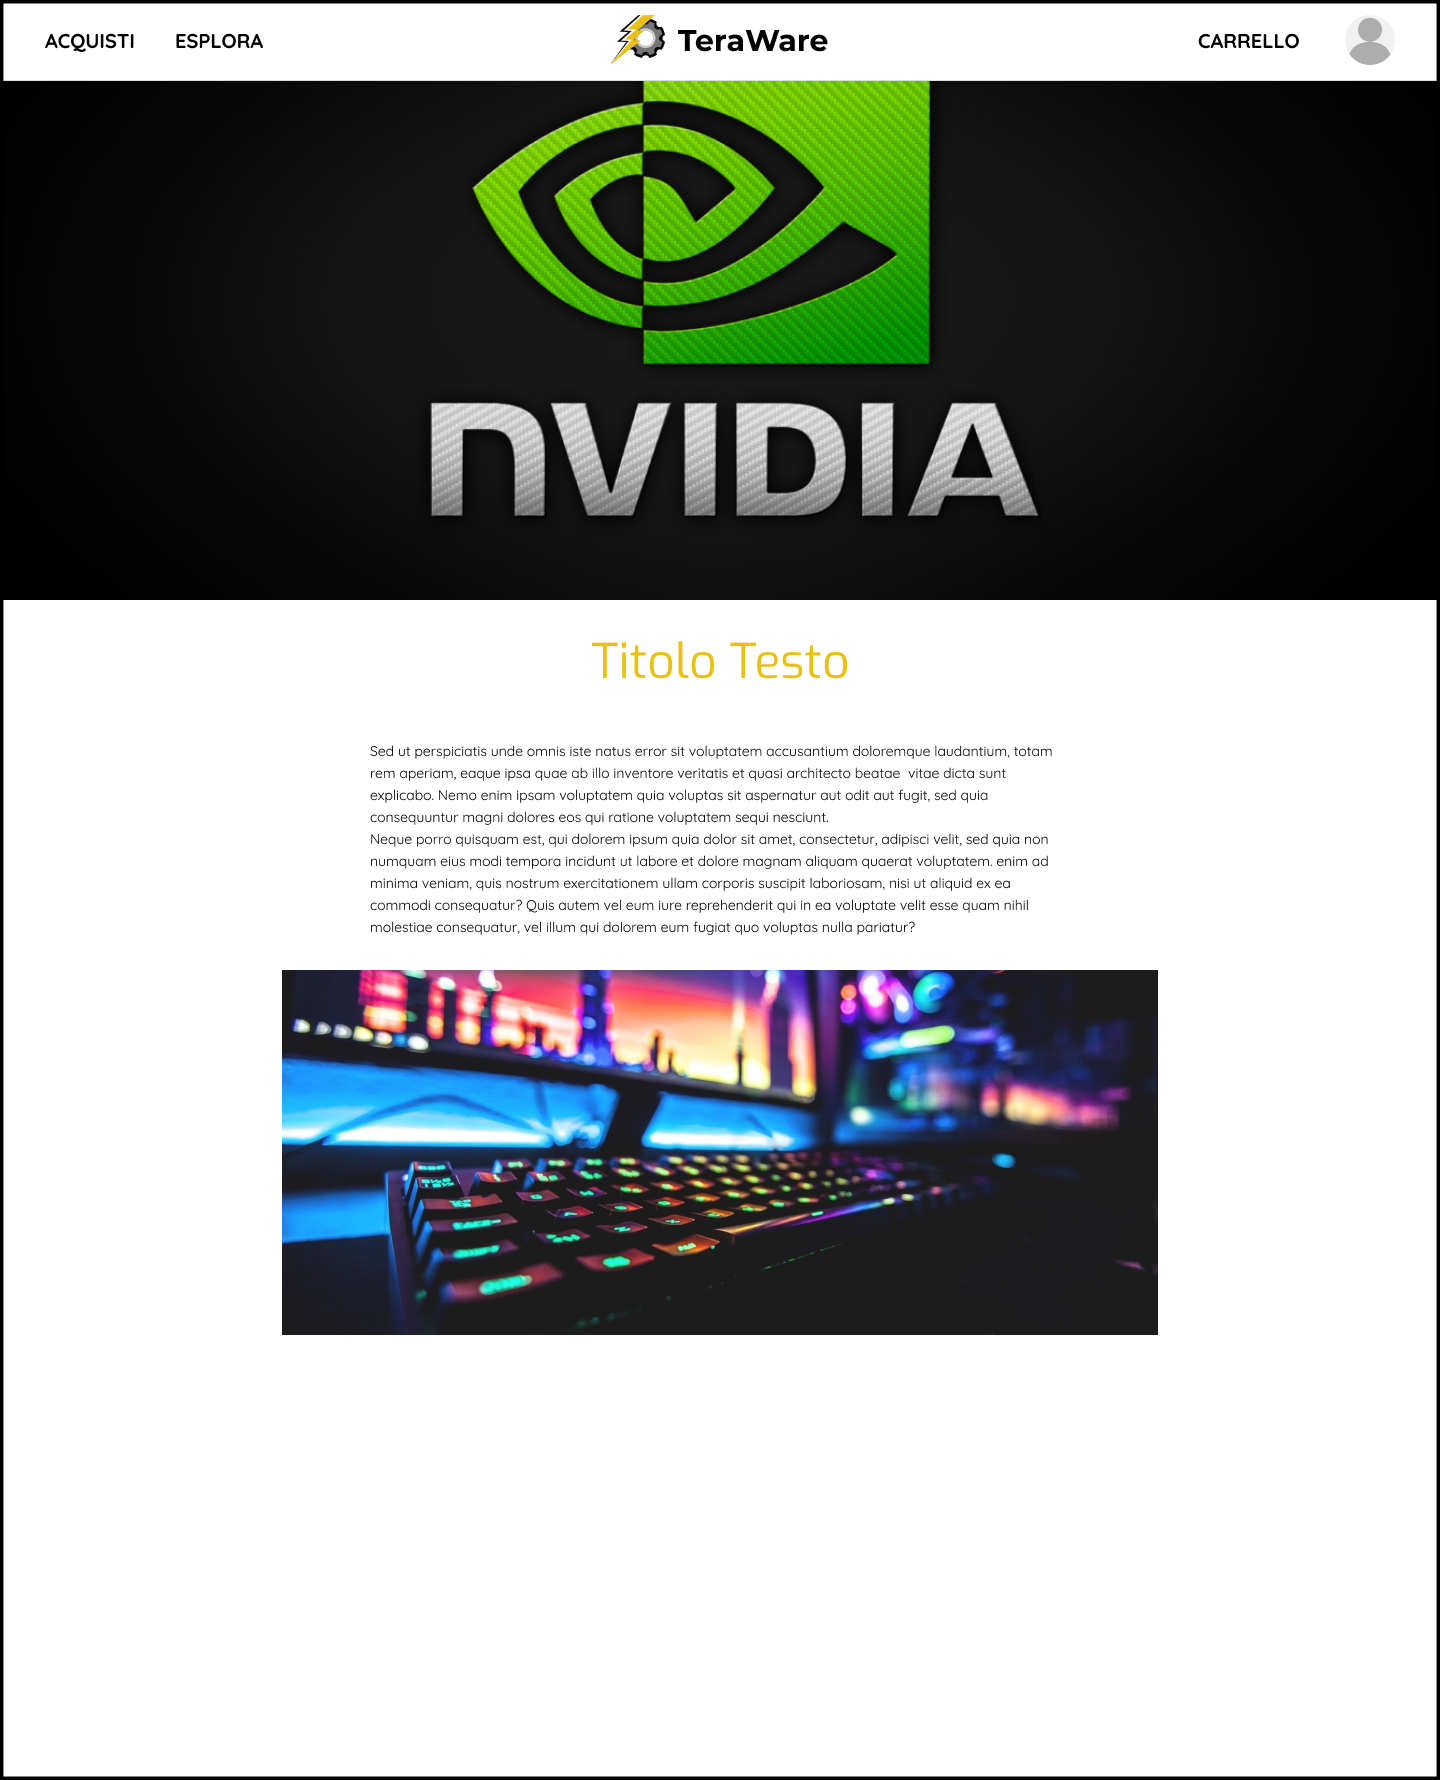
\includegraphics[scale=0.29]{teraware/_layoutnews.png}
            \end{center}
    \section{Tema}
        \begin{center}
        
\includegraphics[scale=0.09]{teraware/vlogo.png}
        \end{center}
    Il tema è scelto attorno a una scala di grigi e un giallo scuro, in modo da rendere visivamente il design consistente con il logo che è presente nella parte alta del sito. Non è presente nessuna immagine di sfondo.
    \section{Scelta dei colori}
        \begin{center}
            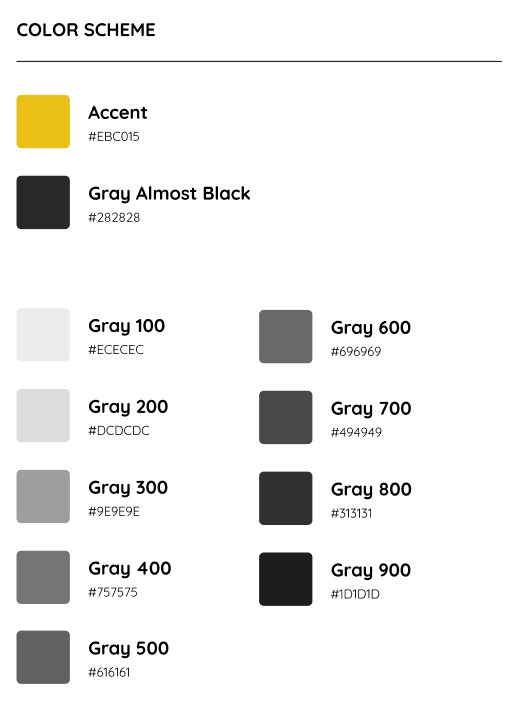
\includegraphics[scale=0.75]{teraware/colors.jpeg} 
        \end{center}
\end{large}
\end{document}